\documentclass[12pt, letterpaper]{article}
\usepackage[utf8]{inputenc}
\usepackage[english]{babel} % To obtain English text with the blindtext package
\usepackage{blindtext}
\usepackage{amsmath}
\usepackage{amssymb}
\usepackage{enumitem}
\usepackage{courier}
\usepackage{listings}
\usepackage{graphicx}
\usepackage{pgfplots}
\graphicspath{ {./images/} }

\lstdefinestyle{mystyle}{
    basicstyle=\fontsize{6}{8}\selectfont\ttfamily,
    breakatwhitespace=false,         
    breaklines=true,                 
    captionpos=b,                    
    keepspaces=true,                 
    numbers=left,                    
    numbersep=5pt,                  
    showspaces=false,                
    showstringspaces=false,
    showtabs=false,                  
    tabsize=2
}

\lstset{style=mystyle}

\title{CSCI2291 Homework 6}
\author{Jack Moffatt}
\date{March 3, 2022}


\begin{document}
\maketitle
\noindent\makebox[\linewidth]{\rule{18cm}{0.4pt}}
\section*{Problem 1}

\begin{enumerate}
    \item [(a)] We will use the following code as a solution:
\begin{lstlisting}[language = python]
    higgs_dataset = skd.fetch_openml("higgs", version=1, as_frame=True)
    data = higgs_dataset.data
    target = higgs_dataset.target

    imp = Imputer(missing_values=np.nan, strategy='mean')
    data = imp.fit_transform(data)

    scaler = StandardScaler()
    data = scaler.fit_transform(data)

    lr = skl.LogisticRegression().fit(data, target)
    score = lr.score(data, target)
    print(f"{'Classification Accuracy:' :<30}{score}")
\end{lstlisting}
    We begining by fetching the {\bf higgs} data set from OpenML. Next, we assign local variables 
    to both the data and target sets. Using the Simple Imputer from {\bf sklearn}, we clean up 
    \texttt{np.nan} values by replacing them with mean values. Then we finish our preprocessing by 
    using the {\bf sklearn} class {\bf StandardScaler}, to standardize that attributes to have a zero mean 
    and a variance of 1.
    Now, we fit a logistic regression to the dataset and target vector. We can see that testing the 
    model over our dataset, we see the following classification accuracy:
\begin{lstlisting}[language = python]
    >>>  Classification Accuracy:      0.6412340642529322
\end{lstlisting}
    We can see that our model has a $65\%$ fit to the dataset, it
    can explain much of the variations in the data, but there is still room for improvement. 
\newpage
    \item [(b)] We will use the following code as a solution:
\begin{lstlisting}[language = python]
    higgs_dataset = skd.fetch_openml("higgs", version=1, as_frame=True)
    data = higgs_dataset.data
    target = higgs_dataset.target
    
    imp = Imputer(missing_values=np.nan, strategy='mean')
    data = imp.fit_transform(data)
    
    scaler = skp.StandardScaler()
    data = scaler.fit_transform(data)
    
    lr = skl.LogisticRegression().fit(data, target)
    cross_score = cross_val_score(lr, data, target, cv=10)
    print(f"{'Cross Scores:' :<20}{cross_score}")   
    print(f"{'Mean: ' :<20}{np.mean(cross_score)}")
    print(f"{'STD Deviation: ' :<20}{np.std(cross_score)}")    
\end{lstlisting}
    We can see that lines $1-11$ are identical to part {\bf a}. Now, in we use the 
    {\bf cross\_val\_score} fucntion in {\bf sklearn} to estimate the generalization
    accuracy of our logistic regression over the dataset. \\ \\
    We will set the number of folds to 10, by specifying the \texttt{cv} parameter. 
    We see that we have the following results:
\begin{lstlisting}[language=python] 
    >>> Cross Scores:       [0.644 0.647 0.638 0.633 0.639 0.645 0.635 0.641 0.646 0.641]
    >>> Mean:               0.641
    >>> STD Deviation:      0.004
\end{lstlisting}
    From these results, we can tell that our generally, our model has a score of $.64$ and is
    very consistent, as the standard deviation is less than $1\%$. 
\newpage
    \item [(c)] We will use the following code as a solution: 
\begin{lstlisting}[language=python]
    higgs_dataset = skd.fetch_openml("higgs", version=1, as_frame=True)
    data = higgs_dataset.data
    target = higgs_dataset.target

    imp = Imputer(missing_values=np.nan, strategy='mean')
    data = imp.fit_transform(data)

    scaler = skp.StandardScaler()
    data = scaler.fit_transform(data)

    lr = skl.LogisticRegression().fit(data, target)
    folds = [2, 4, 8, 16, 32, 64]
    for num in folds:
        cross_score = cross_val_score(lr, data, target, cv=num)
        print(f"-------{num} folds-------")
        print(f"{'Mean: ' :<20}{np.mean(cross_score)}")
        print(f"{'STD Deviation: ' :<20}{np.std(cross_score)}")
\end{lstlisting}
    Again, we see that lines $1-11$ are identical to parts {\bf a} and {\bf b}. 
    This time, after fitting our model, we loop over the list \texttt{[2, 4, 8, 16, 32, 64]}, 
    and we run {\bf cross\_val\_scores} with $k$ number of folds for all $k \in [2, 4, 8, 16, 32, 64]$. 
    Printing our results for each itteration, we see that 
\begin{lstlisting}[language = python]
>>>  Mean:               0.6404385517593065
>>>  STD Deviation:      0.0001325854156042916
>>>  -------4 folds-------
>>>  Mean:               0.6406425368695239
>>>  STD Deviation:      0.003611404142075488
>>>  -------8 folds-------
>>>  Mean:               0.640928017787193
>>>  STD Deviation:      0.003517847016119673
>>>  -------16 folds-------
>>>  Mean:               0.6406832208235512
>>>  STD Deviation:      0.005178623142595439
>>>  -------32 folds-------
>>>  Mean:               0.6407547696450705
>>>  STD Deviation:      0.0076560042992938875
>>>  -------64 folds-------
>>>  Mean:               0.6408055630779084
>>>  STD Deviation:      0.011903801846240437
\end{lstlisting}
    From this experiment, we can see that our mean value stays consistent for any
    number of folds. However, The standard deviation of our accuracy scores increase 
    as we increase the number of folds. This is likely due to the fact that as we increase
    number of "folds" (divisions of the dataset) each of these smaller folds will be smaller 
    and thus more "random".
    This will increase the chance that the models performance will 
    decrease, because the "training set" is smaller and thus more random. This results in more
    deviation among all the indvidual tests, but the mean score remains steady. 
\end{enumerate}

\newpage
\noindent\makebox[\linewidth]{\rule{18cm}{0.4pt}}
\section*{Problem 2}
\begin{enumerate}
    \item [(a)] We will use the following code as a solution:
\begin{lstlisting}[language=python]
    higgs_dataset = skd.fetch_openml("higgs", version=1, as_frame=True)
    data = higgs_dataset.data
    target = higgs_dataset.target

    imp = Imputer(missing_values=np.nan, strategy='mean')
    data = imp.fit_transform(data)

    scaler = StandardScaler()
    data = scaler.fit_transform(data)

    lr = LogisticRegression().fit(data, target)
    dtc = DecisionTreeClassifier().fit(data, target)
    lr_score = cross_val_score(lr, data, target, cv=10)
    dtc_score = cross_val_score(dtc, data, target, cv=10)

    plt.boxplot([lr_score, dtc_score], positions=[-1, 1],
                labels=["Logistic Regression", "Decision Tree Classifier"])
    plt.ylim([.6, .7])
    plt.ylabel("Cross Validation Scores with 10 Folds")
    plt.title("Logistic Regression vs. Decision Tree Classifier\nCross Validation Scores")
    plt.show()
\end{lstlisting}
    Again, lines $1-11$ are identical to problem {\bf 1}. Then, we additionally fit 
    a {\bf DecisionTreeClassifier} model to the dataset and cross validate each model 
    using {\bf cross\_val\_score} with 10 folds. We then create a boxplots for each of 
    our sets of 10 scores. After applying the appropriate labels and scaling, we see 
    \[
        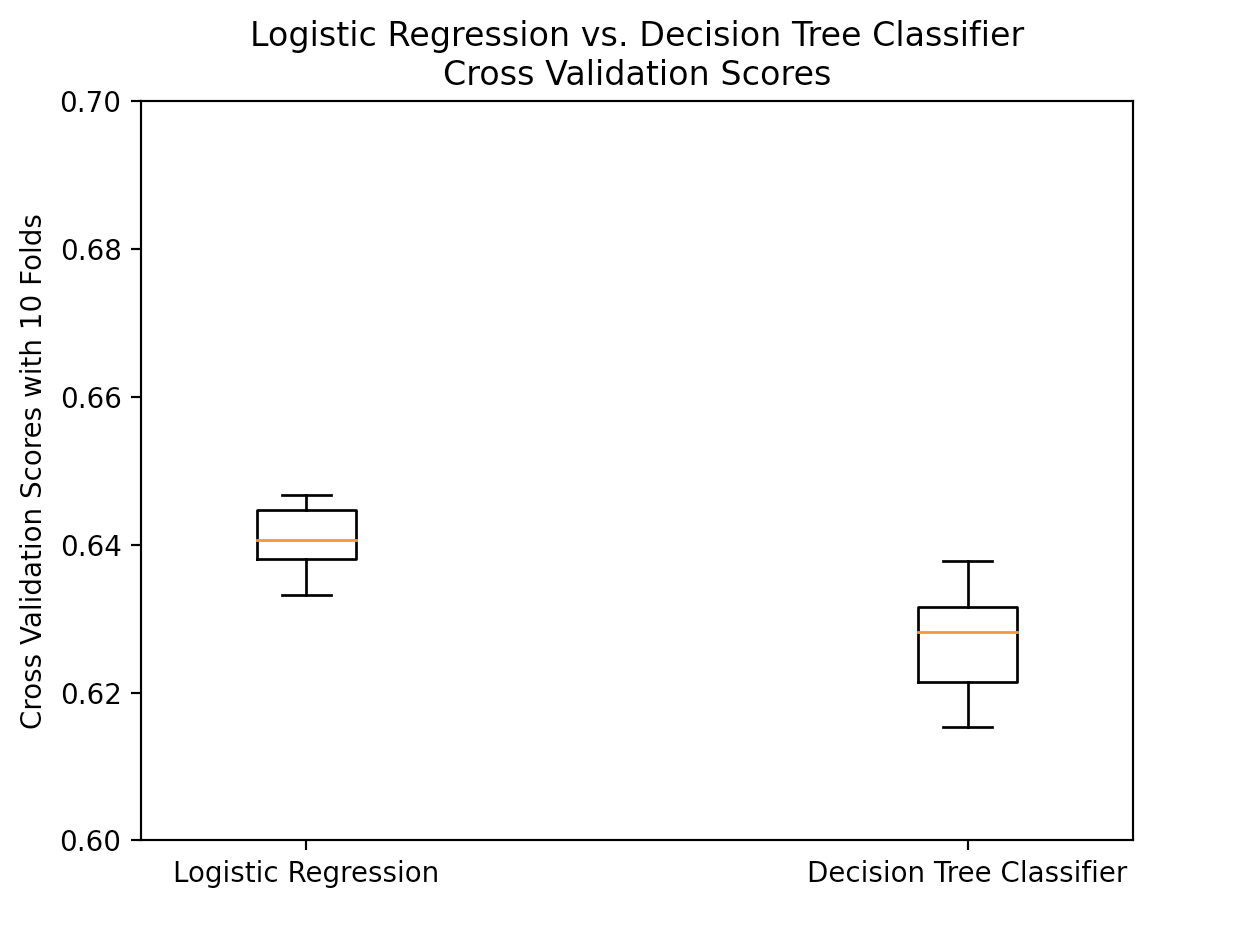
\includegraphics[scale = .33]{images/boxplot_6a.png}
    \]  
    This boxplot helps provide very useful insight into our results. We can clearly see that
    the mean of the Logistic Regression is slightly higher, but only by a difference of approximatley $1\%$
    or so. However, we can tell the the height of the Decision Tree Classifier is greater, which tells us that 
    the Decision Tree Classifier has a higher standard deviation. This suggests that any given
    Decision Tree Classifier model is more likely to have be less accurate than any single Logistic Regression 
    model. This is likely due to the methods used to create the models. Namely, the method used to 
    generate the Decision Tree model enhances the specific noise of the training set, more so than 
    the Logistic Regression models. 
\newpage
    \item [(b)] We will use the following code as solution:
\begin{lstlisting}[language=python]
    higgs_dataset = skd.fetch_openml("higgs", version=1, as_frame=True)
    data = higgs_dataset.data
    target = higgs_dataset.target
    
    imp = Imputer(missing_values=np.nan, strategy='mean')
    data = imp.fit_transform(data)
    
    scaler = StandardScaler()
    data = scaler.fit_transform(data)
    
    lr = LogisticRegression().fit(data, target)
    dtc = DecisionTreeClassifier().fit(data, target)
    lr_score = cross_val_score(lr, data, target, cv=10)
    dtc_score = cross_val_score(dtc, data, target, cv=10)
    
    lr_score_stand = scaler.fit_transform(lr_score.reshape(-1, 1))[:, 0]
    dtc_score_stand = scaler.fit_transform(dtc_score.reshape(-1, 1))[:, 0]
    
    test_stand = ttest_ind(lr_score_stand, dtc_score, equal_var=True)
    print(f"{'t-statistic:' :<20}{test_stand[0]}")
    print(f"{'p-value:' :<20}{test_stand[1]}")
\end{lstlisting}
    Again, lines $1-11$ are the same as above. We next calculate the {\bf cross\_val\_score} for each model. 
    Then, we standardize the scores using the standard scaler. The arrays must be reshaped to 2D arrays to use 
    the scaler, and then we take the column vector to pass to our test. \\ \\
    We can use a indpendent t-test, to calculate weather the variations in the means between the two scoresets 
    are due to random chance. Printing our results we see that
\begin{lstlisting}[language=python]
    >>>  t-statistic:        -1.8796393366850002
    >>>  p-value:            0.07644491368115493
\end{lstlisting}
    We can see that the p-value is very close to 0. Thus, this tells us that there is a very low probability 
    that the variations in the means of the two sets are due to random chance. From this test we can conclude 
    that the difference in means of the {\bf cross\_cal\_scores} sets is unlikely to be a result of random chance. 
\end{enumerate}

\newpage
\noindent\makebox[\linewidth]{\rule{18cm}{0.4pt}}
\section*{Problem 3}
\begin{enumerate}
    \item [(a)] We can set up 3 indepedent trials. The probability of success is $p=0.2$, while the probability
    failure is $0.8$. Let $X_i$ be the event that the $i^{th}$ trial is a 
    success. Since these, trials are indepedent, we know that 
    \begin{align*}
        P(X_1 \cap X_2 \cap X_3) &= P(X_1) \cdot P(X_2) \cdot P(X_3) \\
        &= 0.2 \cdot 0.2 \cdot 0.2 = 0.2 ^ 3 = 0.008
    \end{align*}
    So, we conclude that the probability of the model correctly predicting all three class labels is $0.008$.
    \item [(b)] Let $X$ be the number of correct predictions that the model makes in 10 trials. Then we state that 
    \[
        X \thicksim \text{Binom}(n, p)
    \]
    where $n=10$ and $p = 0.2$. Then, we can compute the probability that it will make $7$ correct 
    classifications:
    \begin{align*}
        P(x = 7) &= \binom{10}{7}p^7(p-1)^3 \\
        &= (120)(0.2)^7(0.8)^3 \\
        &= (120)(0.0000128)(0.512)\\
        &= (120)(0.0000065536)\\
        &= (0.000786432)
    \end{align*}
    So we see that probability of the model will make 7 correct predictions in a set of 10 classifications is 
    $0.079\%$
\end{enumerate}

\newpage
\noindent\makebox[\linewidth]{\rule{18cm}{0.4pt}}
\section*{Problem 4}
\begin{enumerate}
    \item [(a)] The current performance of AI-based algorithims still needs improvement. As stated in the article, 
    "Given that automatic screening tools are actively being developed in research19,20,21,22,23 and have been shown 
    to match specialist performance16, underdiagnosis in AI-based diagnostic algorithms can be a crucial concern if 
    used in the clinical pipeline for patient triage." It is clear that progress has been made in the effort to utilize
    AI in the medical world, however, there is still a concern over the accuracy of the algorithims at this time, and their 
    current rate of underdiagnosis could cause problems. 
    \item [(b)] Misdiagnosis is when a patient is diagnosed with a condition, but it is labeled as less severe 
    than it actually is. Conversely, underdiagnosis is when a patient is deemed to be healthy, when really they 
    need medical attention. As stated in the paper, underdiagnosis is far more troubling as "underdiagnosis is 
    potentially worse than misdiagnosis, because in the latter case, the patient still receives clinical care, 
    and the clinician can use other symptoms and data sources to clarify the mistake". 
    \item [(c)] As described in the paper, the term false-positive rate, is the rate at which the algorithims 
    incorrectly assign the "no finding" label to patients. In other words, the {\bf FPR} measures the rate at which patients 
    are underdiagnosed by AI algorithims.
    \item [(d)] Gender, age, race, and socieo-econmoic status all played a role in the underdiagnosis rates of the 
    algorithims. According to {\bf Fig.2a}, which shows the results for false-postive rates sorted by various status traits, 
    the FPR for males was approximatley $20\%$, while it was closer to $25\%$ for females. Additionally, patients in the 
    age range of $0-20$ years old had an FPR of approximatley $45\%$. The false-positive rate for blacks and hispanics was 
    around $10\%$ higher than for other races. And, finally, those on medicaid had approximatley a $10\%$ higher FPR, than 
    patients on private insurance policies. 
    \item [(e)] The article makes it quite clear that much of the bias that is present in the datasample and then amplified 
    by the algorithims, stems from the original diagnoses from which the dataset was created. This is likely a result of the 
    inaccessability of healthcare ot underserved groups: "Patients with low socioeconomic status may have fewer interactions 
    with the healthcare system, or they may be more likely to visit a teaching or research clinic where clinical reasoning or 
    treatment plans may be different". \\ \\
    Additionally, looking at the table summary of all statistics, we see that the proportions of race present in the dataset, do not
    correspond to the ratial distribution of the 2020 US census: 
    \begin{center}
            \begin{tabular}{c || c | c}
            Race & Data Set & US Census \\
            \hline \hline
            Asian &  3.2 \% & 5.9\% \\
            \hline
            Black & 18.6 \% &  12.1\%\\
            \hline
            Hispanic & 6.4 \%& 18.7\% \\
            \hline
            Native & 0.3 \% & 0.2\% \\
            \hline
            White & 67.6 \% & 57.8 \% \\
            \hline
            Other & 3.8 \% & 0.5\%
            \end{tabular}   
    \end{center}
    We can see that Whites and Blacks are over represented relative to the population, while Asians and Hispanics are under represented 
    in the data set used for the AI algorithims. This definetley can lead to a bias in the model, when it is used on the entire population, 
    because the model may be skewed to better diagnosis a white patient, rather than a patient of another race. 
\end{enumerate}
\end{document}